\documentclass[11pt]{article}
\usepackage{amsfonts,amssymb,amsmath,amsthm,amscd}
\usepackage{courier}
\usepackage{mathtools}
\usepackage{fancyhdr}
\usepackage{enumitem}
\usepackage{newtxtext,newtxmath}
\usepackage{listings}
\usepackage{wasysym}
\usepackage{makecell}
\usepackage[linesnumbered,ruled]{algorithm2e}
\usepackage[margin=2.5cm]{geometry}
\parindent 0px

%Header
\fancyhf{}
\setlength{\headheight}{50pt}
\pagestyle{fancy}
\lhead{04/27/2022}
\chead{\bf\LARGE Final Writeup}
\rhead{Yu-Kai Wang, Matthew Uryga\\CSCI-4969\\Spring 2022}
\cfoot{\thepage}
\headsep 5mm

%Document
\allowdisplaybreaks

%List set
\lstset{frame=tb, language=python, basicstyle={\small\ttfamily}}

%Functions
\newcommand{\prob}[1]{{\Large\textbf{#1}}}
\newcommand{\npr}{\\[8mm]}
\newcommand{\itm}[1]{\item[(#1)]}
\newcommand{\np}{\newpage}
\newcommand{\N}{\mathbb{N}}
\newcommand{\Z}{\mathbb{Z}}
\newcommand{\Q}{\mathbb{Q}}
\newcommand{\R}{\mathbb{R}}
\newcommand{\C}{\mathbb{C}}
\newcommand{\D}{\mathcal{D}}
\newcommand{\PP}{\mathbb{P}}
\newcommand{\HH}{\mathcal{H}}
\newcommand{\PPT}[1]{\PP(\text{#1})}
\newcommand{\E}{\mathbb{E}}
\newcommand{\ET}[1]{\E[\text{#1}]}
\newcommand{\Lang}{\mathcal{L}}
\newcommand{\pminf}{_{-\infty}^{+\infty}}
\newcommand{\schrodeq}{-\frac{\hslash^2}{2m}\PPartial{\Psi(x,t)}{x}+V(x)\Psi(x,t)=i\hslash\Partial{\Psi(x,t)}{t}}
\newcommand{\st}{^{*}}
\newcommand{\Claim}{{\bf Claim: }}
\newcommand\sbullet[1][1]{\mathbin{\ThisStyle{\vcenter{\hbox{%
	\scalebox{#1}{$\SavedStyle\bullet$}}}}}%
}
\newcommand*\circled[1]{\tikz[baseline=(char.base)]{
						\node[shape=circle,draw,inner sep=1pt] (char) {#1};}}
\newcommand{\hs}{\hslash}
\newcommand{\eiet}[1]{e^{\frac{iE_{#1}t}{\hslash}}}
\newcommand{\neiet}[1]{e^{-\frac{iE_{#1}t}{\hslash}}}
\newcommand{\eikx}[1]{e^{ik_{#1}x}}
\newcommand{\neikx}[1]{e^{-ik_{#1}x}}
\newcommand{\pr}{^\prime}
\newcommand{\ppr}{^{\prime\prime}}
\newcommand{\pppr}{^{\prime\prime\prime}}
\newcommand{\ppppr}{^{\prime\prime\prime\prime}}
\newcommand{\op}[1]{\hat #1}
\newcommand{\dg}{^\dagger}
\newcommand{\lal}{(\alph*)}
\newcommand{\lrom}{(\roman*)}
\newcommand{\lara}{(\arabic*)}
\newcommand{\comm}[2]{\left[\hat{#1},\hat{#2}\right]}
\newcommand{\xyz}{(x,y,z)}
\newcommand{\bbar}[1]{\mkern 1.5mu\overline{\mkern-1.5mu#1\mkern-1.5mu}\mkern 1.5mu}
\newcommand{\dx}{\,dx}
\newcommand{\oneminus}[1]{\left(1-#1\right)}
\newcommand{\hi}{\frac{\hs}{i}}
\newcommand{\ih}{\frac{i}{\hs}}
\newcommand{\e}[1]{\cdot10^{#1}}
\newcommand{\hv}{\inv{2}}
\newcommand{\inv}[1]{\frac{1}{#1}}
\newcommand{\invsq}[1]{\frac{1}{\sqrt{#1}}}
\newcommand{\sqfr}[2]{\sqrt\frac{#1}{#2}}
\newcommand{\Partial}[2]{\frac{\partial #1}{\partial #2}}
\newcommand{\PPartial}[2]{\frac{\partial^2 #1}{\partial #2^2}}
\newcommand{\FPartial}[2]{\frac{\partial}{\partial #2}#1}
\newcommand{\FPPartial}[2]{\frac{\partial^2}{\partial #2^2}#1}
\newcommand{\FpPartial}[2]{\frac{\partial}{\partial #2}\left(#1\right)}
\newcommand{\FpPPartial}[2]{\frac{\partial^2}{\partial #2^2}\left(#1\right)}
\newcommand{\deriv}[2]{\frac{d #1}{d #2}}
\newcommand{\dderiv}[2]{\frac{d^2 #1}{d #2^2}}
\newcommand{\expval}[1]{\left\langle #1 \right\rangle}
\newcommand{\vvatrix}[2]{\paren{\begin{matrix}#1\\#2\end{matrix}}}
\newcommand{\vvvatrix}[3]{\paren{\begin{matrix}#1\\#2\\#3\end{matrix}}}
\newcommand{\vvvvatrix}[4]{\paren{\begin{matrix}#1\\#2\\#3\\#4\end{matrix}}}
\newcommand{\hhatrix}[2]{\paren{\begin{matrix}#1&#2\end{matrix}}}
\newcommand{\hhhatrix}[3]{\paren{\begin{matrix}#1&#2&#3\end{matrix}}}
\newcommand{\hhhhatrix}[4]{\paren{\begin{matrix}#1&#2&#3&#4\end{matrix}}}
\newcommand{\mmatrix}[4]{\paren{\begin{matrix}#1&#2\\#3&#4\end{matrix}}}
\newcommand{\mmmatrix}[9]{\paren{\begin{matrix}#1&#2&#3\\#4&#5&#6\\#7&#8&#9\end{matrix}}}
\newcommand{\ccases}[4]{\begin{cases}#1&#2\\#3&#4\end{cases}}
\newcommand{\norm}[1]{\left|\left|#1\right|\right|}
\newcommand{\paren}[1]{\left(#1\right)}
\newcommand{\eps}{\epsilon}
\newcommand{\magn}[1]{\left|\left|#1\right|\right|}
\newcommand{\bs}[1]{\boldsymbol{#1}}
\newcommand{\mh}{m_{\HH}}
\newcommand{\dvc}{{d_{VC}}}
%Constants 
\newcommand{\h}{6.626\e{-34}}
\newcommand{\elec}{1.6\e{-19}}
\newcommand{\elecmass}{9.109\e{-31}}  
\newcommand{\cc}{3\e{8}}
%Misc
\DeclarePairedDelimiter\ceil{\lceil}{\rceil}
\DeclarePairedDelimiter\floor{\lfloor}{\rfloor}

\begin{document}
\section{Distribution of Work}
\subsection{Yu-Kai (Steven) Wang}
\begin{enumerate}[label=(\alph*)]
	\item Multihead self attention
	\item Outer product mean
	\item Triangular self attention
	\item IPA Module
	\item Parallelization of model so that it can run on any number of GPUs
	\item Dispatching jobs to the DCS cluster
	\item Optimization of evoformer trunk and structure module
\end{enumerate}

\subsection{Matthew Uryga}
\begin{enumerate}[label=(\alph*)]
	\item Input feature projections
	\item Evoformer trunk structure
	\item Structure module, excluding the IPA module
	\begin{enumerate}[label=(\roman*)]
		\item Backbone update
		\item FAPE and torsion angle loss
		\item etc.
	\end{enumerate}
	\item Dataset for batching of crops for training/validation and whole sequences for testing
	\item Model training and validation loops
	\item Model evaluation
	\item Predicted/Ground truth structure visualization
	\item Writeups
\end{enumerate}

\subsection{Repository Link}
The code for our implementation of Alphafold2 can be found here:\\https://github.com/mnuryga/MLBinfCapstone.
\np

\section{Method}
\subsection{Overall Implementation}
For the most part, the Alphafold2 supplemental paper was followed closely when implementing the model structure.  Some deviations include a reduced breadth of input data (no extra msa information) and some slight variations in the final computation of coordinates.  It is also worth noting that the model was not designed to predict anything beyond the $\phi$ and $\psi$ torsion angles and the locations of $C$, $C_{\alpha}$, and $N$. 

\subsection{Parameters}
Due to memory, time, and processing power limitations, the parameters of the model were decreased from the specifications in the Alphafold2 paper.  Namely, the following parameters were altered:
\begin{flalign*}
	N_{res} &= 256 \longrightarrow 64&\\
	N_{clust} &= 16 \longrightarrow 8\\
	c_{m} &= 256 \longrightarrow 128\\
	c_{z} &= 128 \longrightarrow 64\\
	c_{z} &= 128 \longrightarrow 64\\
	c_{MHSA} &= 32 \longrightarrow 16\\
	c_{outer\;prod\;mean} &= 32 \longrightarrow 16\\
	c_{trangular\;attn} &= 32 \longrightarrow 16
\end{flalign*}
Without these parameter reductions, evaluation of the model would not be possible on the largest test sequences, as the GPUs would run out of memory to hold the entirety of the protein and its representations.

\subsection{Tuning of Learning Rate}
Because training took a significant amount of time, the learning rate could not be optimally tuned.  It was determined through short validation runs that a learning rate of 0.001 would be reasonable.  The learning rate was manually halved every 6 epochs.

\subsection{Tuning of Dimension Parameters}
Through a variety of limited experiments, it was found that decreasing the dimension parameters had a minimal effect on the performance of the model, however this may not have been the case in actuality.

\subsection{Training}
Training was conducted on the DCS cluster so that the model could make use of 4 GPUs.  This substantially decreased the training time from approximately 3.5 hours per epoch to 50 minutes per epoch.  In total, the model was trained for 18 epochs.

\subsection{Validation}
Validation was run after each epoch, and the model training was stopped if the validation loss was greater than the 5-epoch rolling mean of previous validation losses, although this never occurred.

\section{Results}
\subsection{Test Loss}
The calculated average test loss was 1.171323 per sequence.\\[2mm]
Below are a couple of plots detailing a few more statistics with the test loss:\\[2mm]

\begin{minipage}{0.45\textwidth}
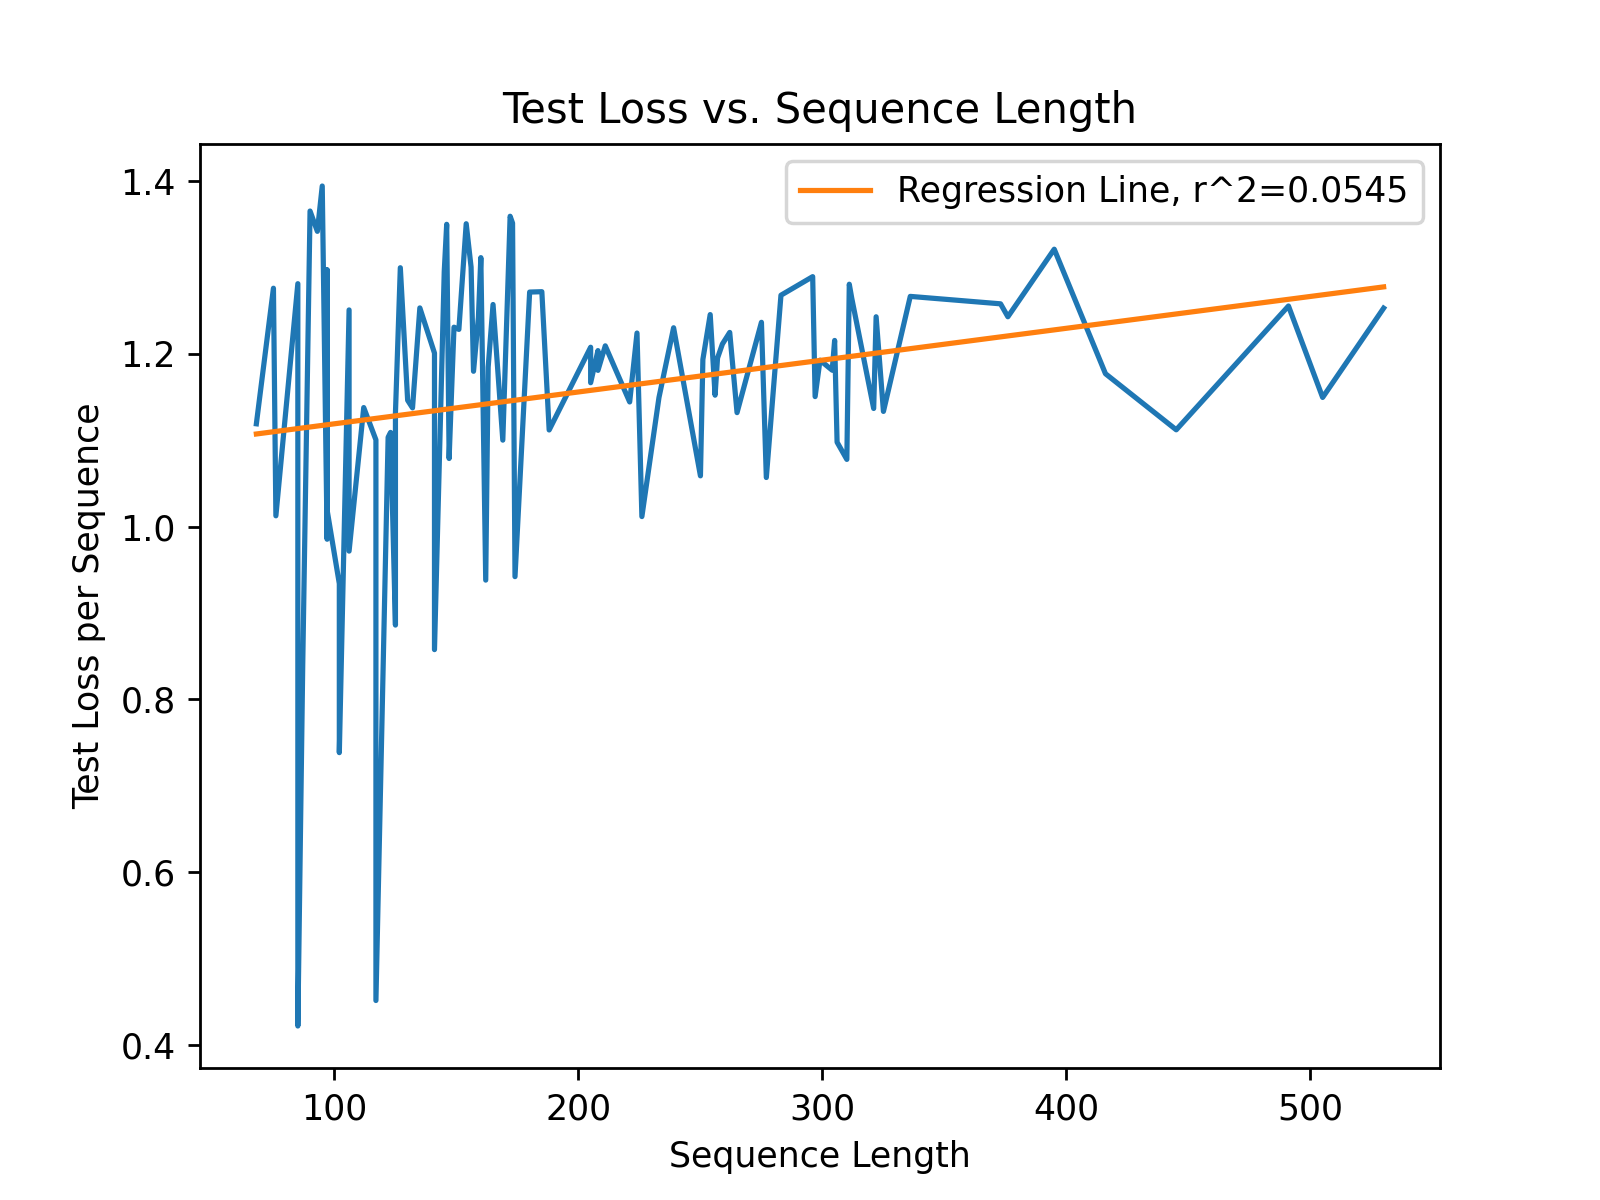
\includegraphics[scale=0.5]{loss_seqs.png}
\end{minipage}
\hfill
\begin{minipage}{0.45\textwidth}
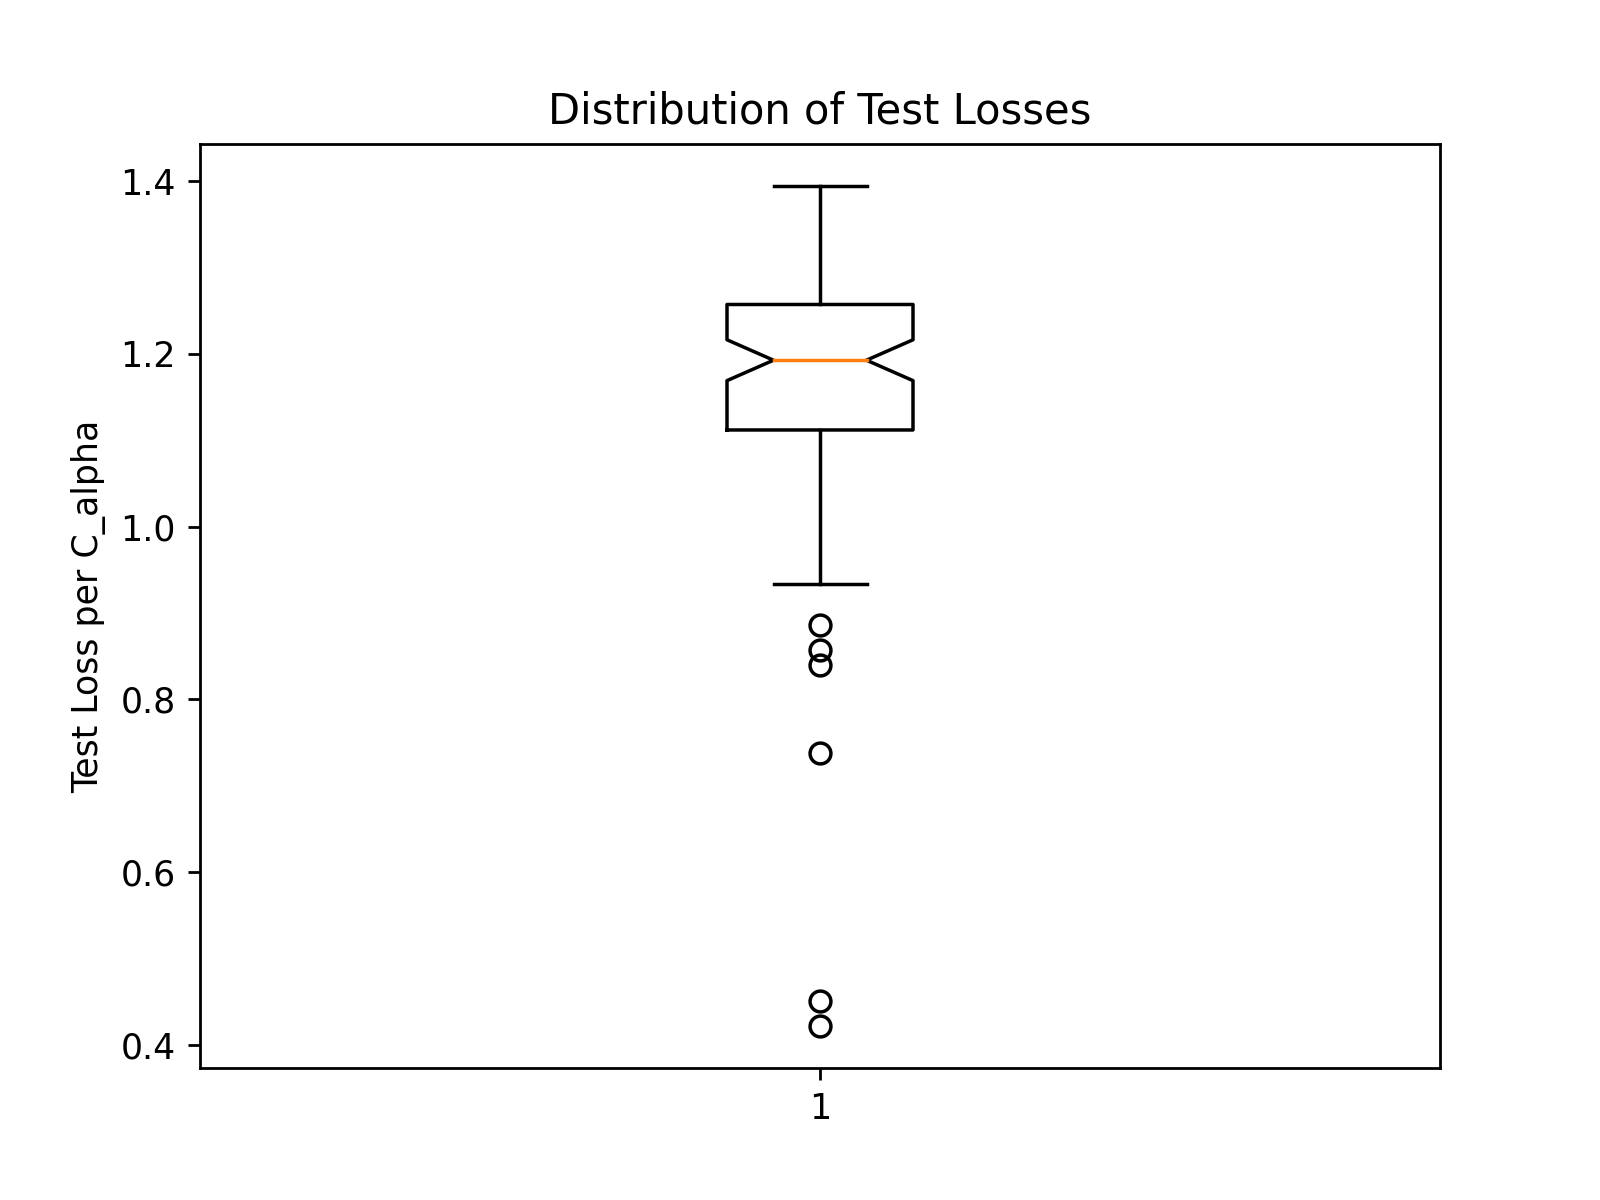
\includegraphics[scale=0.5]{loss_boxplot.png}
\end{minipage}\\[2mm]
From the plots above, it appears that the average loss per sequence does not have a significant correlation with sequence length - the least squares regression line has a $r^{2}$ value of $0.0545$

\section{Visualization}
The predicted and true protein structures were visualized by plotting the coordinates of the $C_{\alpha}$ atoms in 3D-space.\\[2mm]
Below are three sequences that were chosen based on their average loss per sequence (the maximum, median, and minimum average loss sequences).\\[2mm]
For each protein displayed below, there are two 3D-plots: one without reordering and one with reordering.  Reordering was implemented by starting with the first $C_{\alpha}$ in a sequence and selecting the next $C_{\alpha}$ by smallest Euclidean distance.  This is repeated for the entire sequence.\\
This creates a less cluttered plot that allows the similarities/dissimilarities to show more clearly.
\np

\subsection{Best Prediction}
Loss per sequence: $0.42200$.\\[3mm]
Without reordering:\\[2mm]
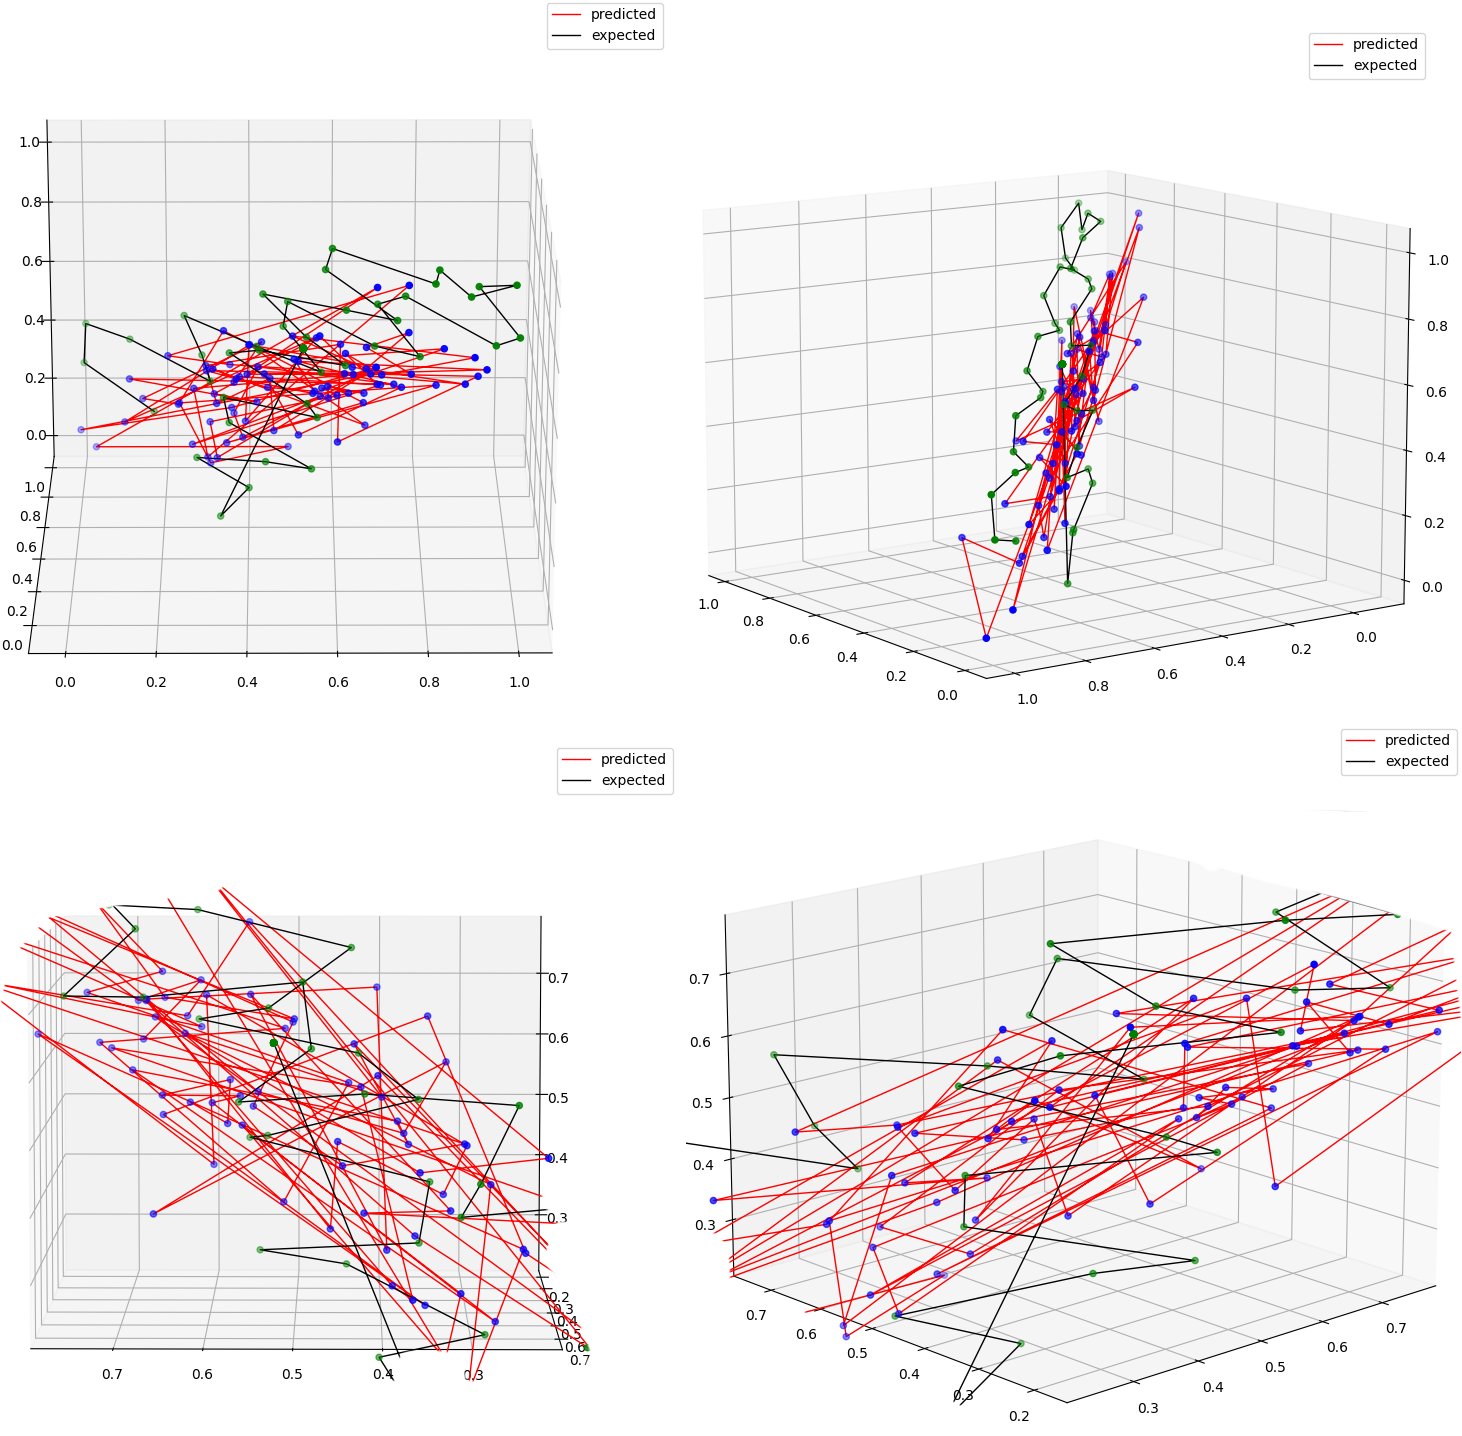
\includegraphics[scale=0.42]{best1.png}\np
With reordering:\\[2mm]
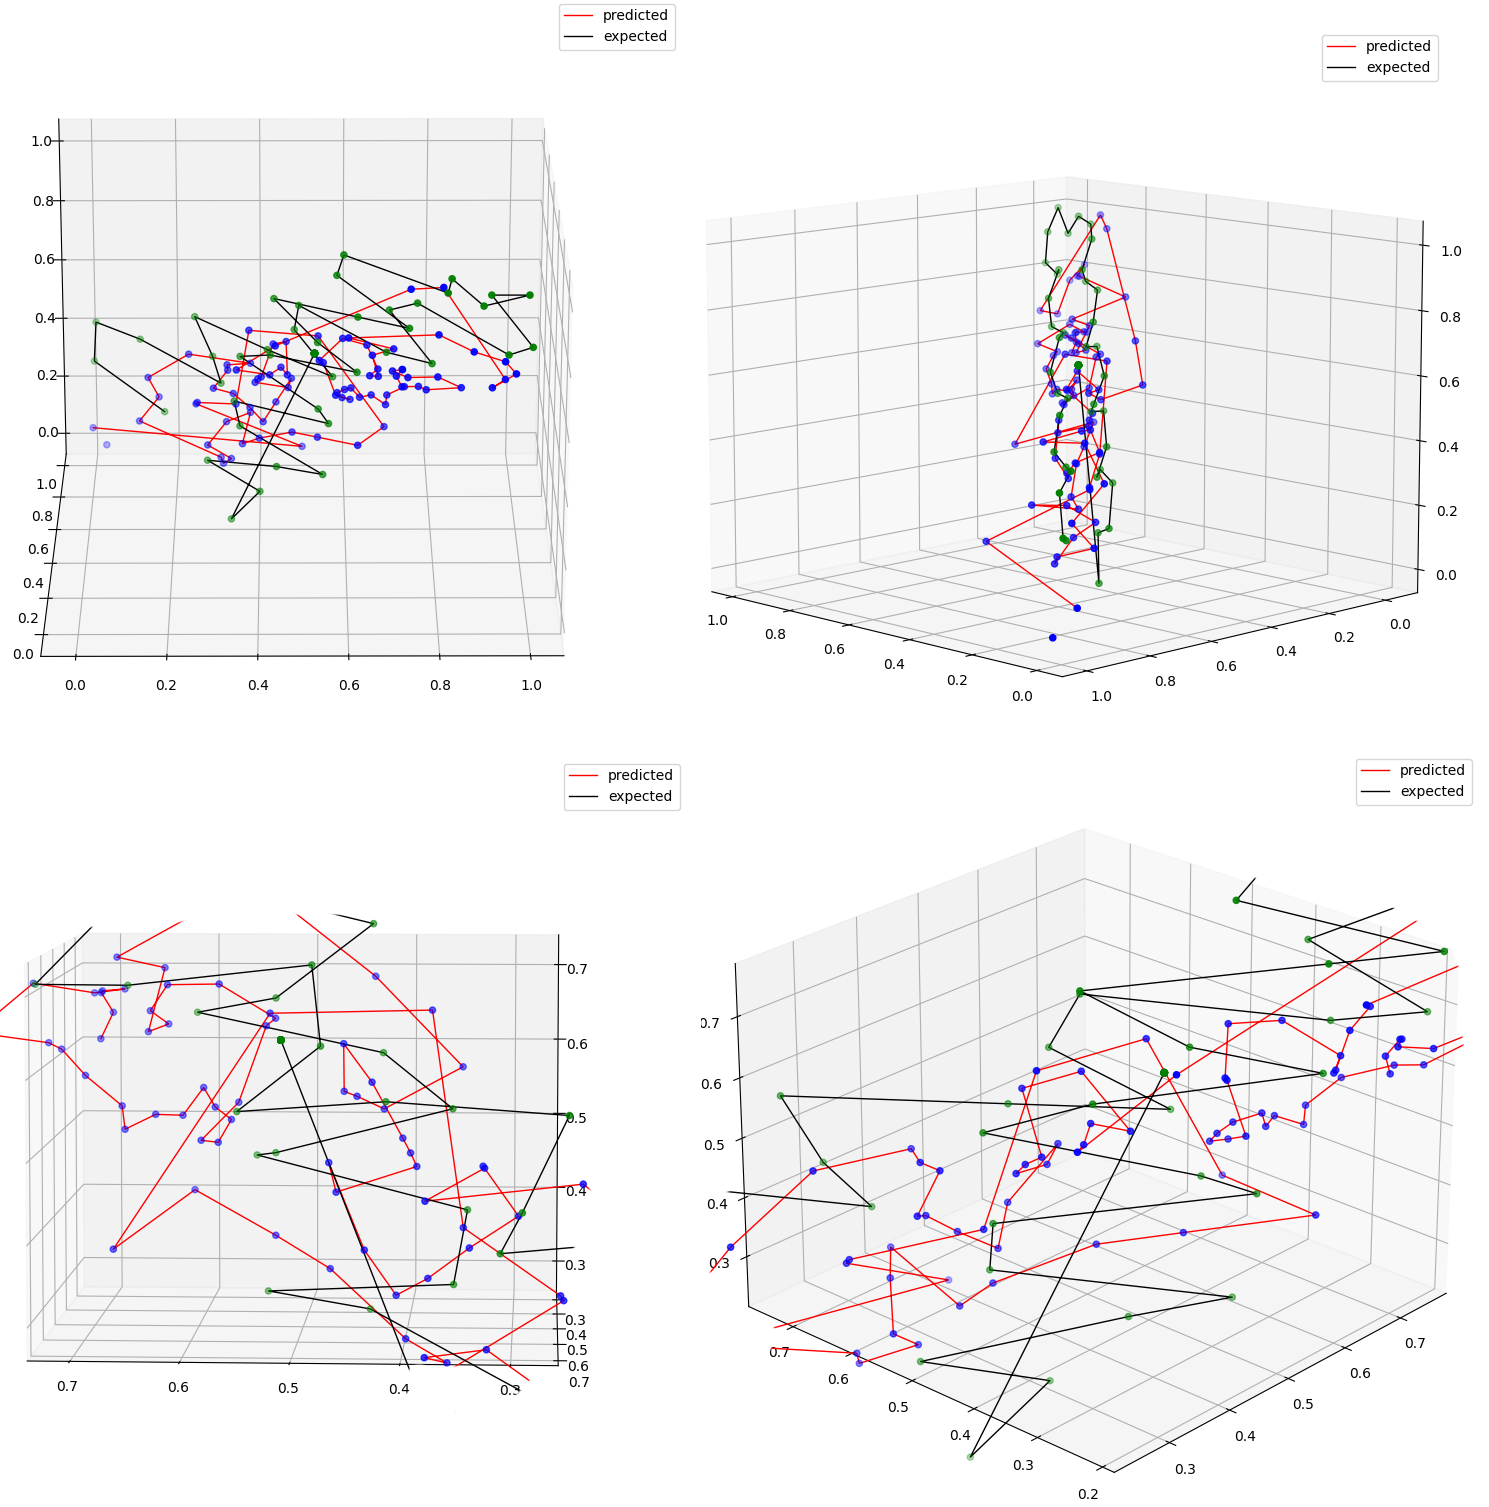
\includegraphics[scale=0.42]{best2.png}\np

\subsection{Median Prediction}
Loss per sequence: $1.17614$.\\[3mm]
Without reordering:\\[2mm]
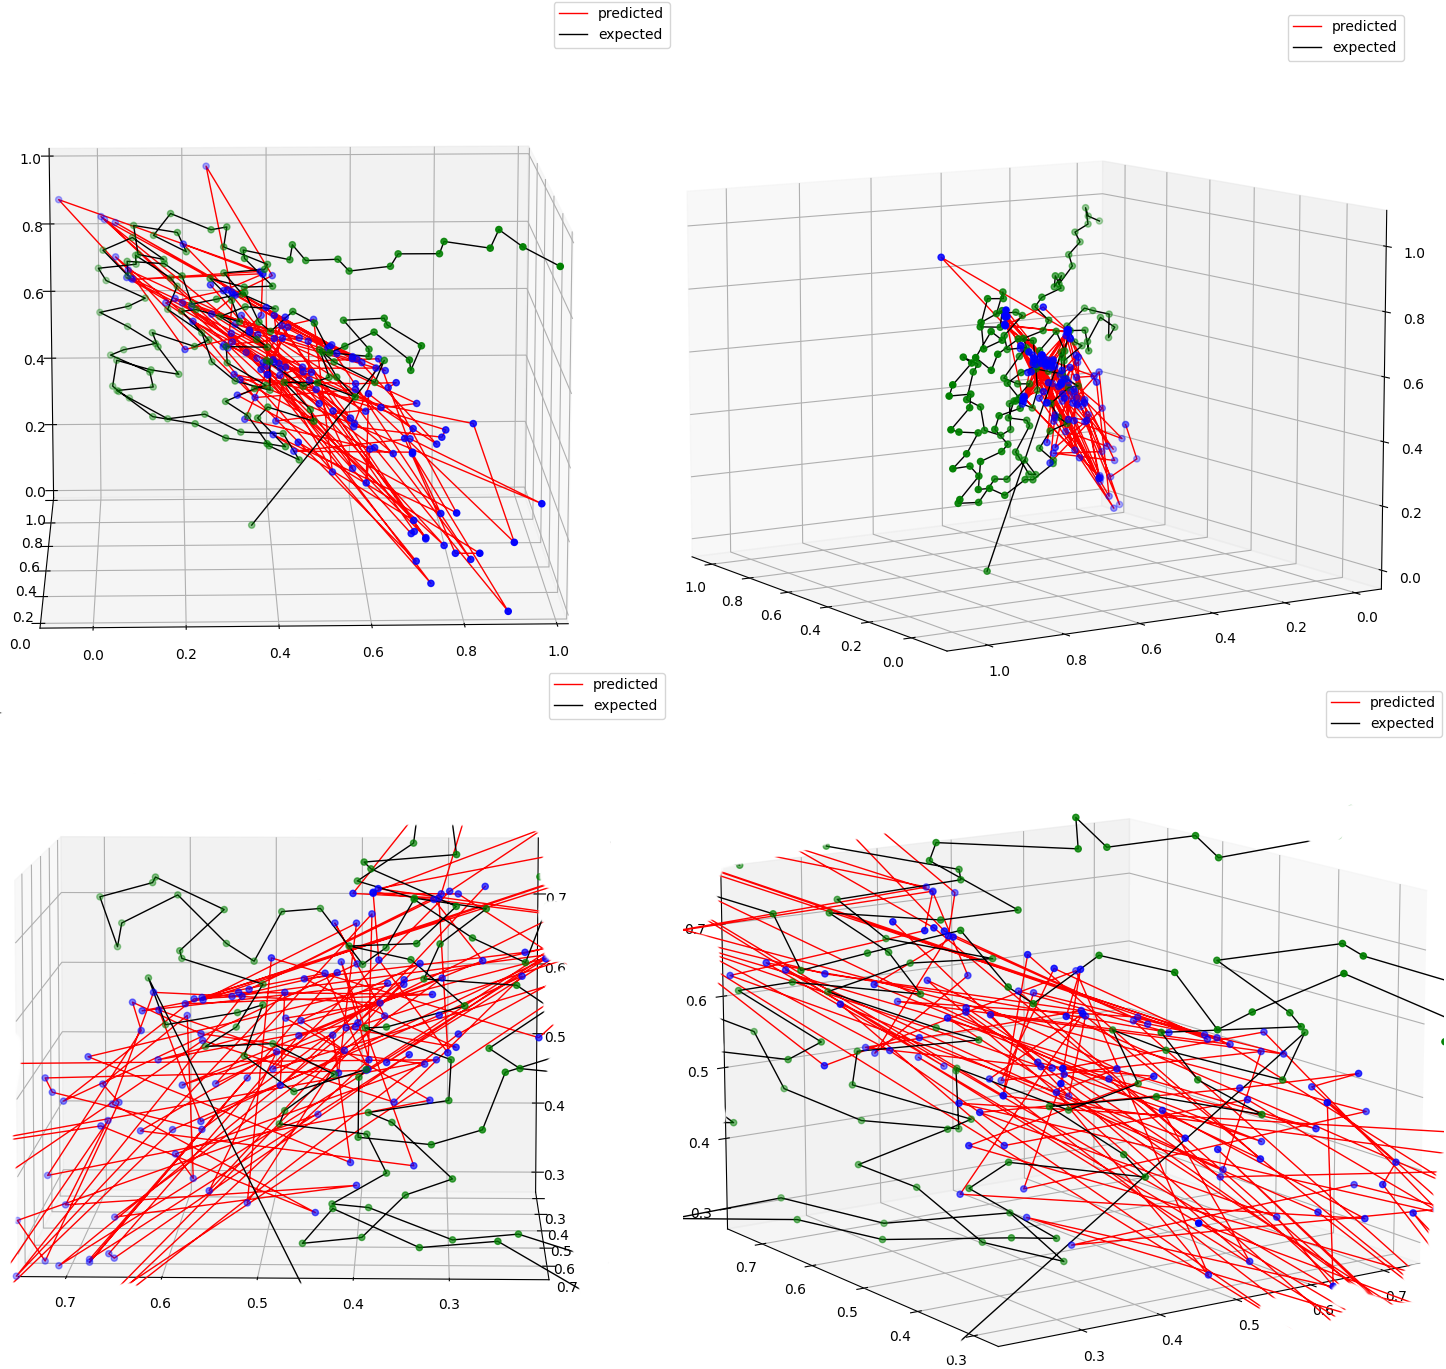
\includegraphics[scale=0.42]{med1.png}\np
With reordering:\\[2mm]
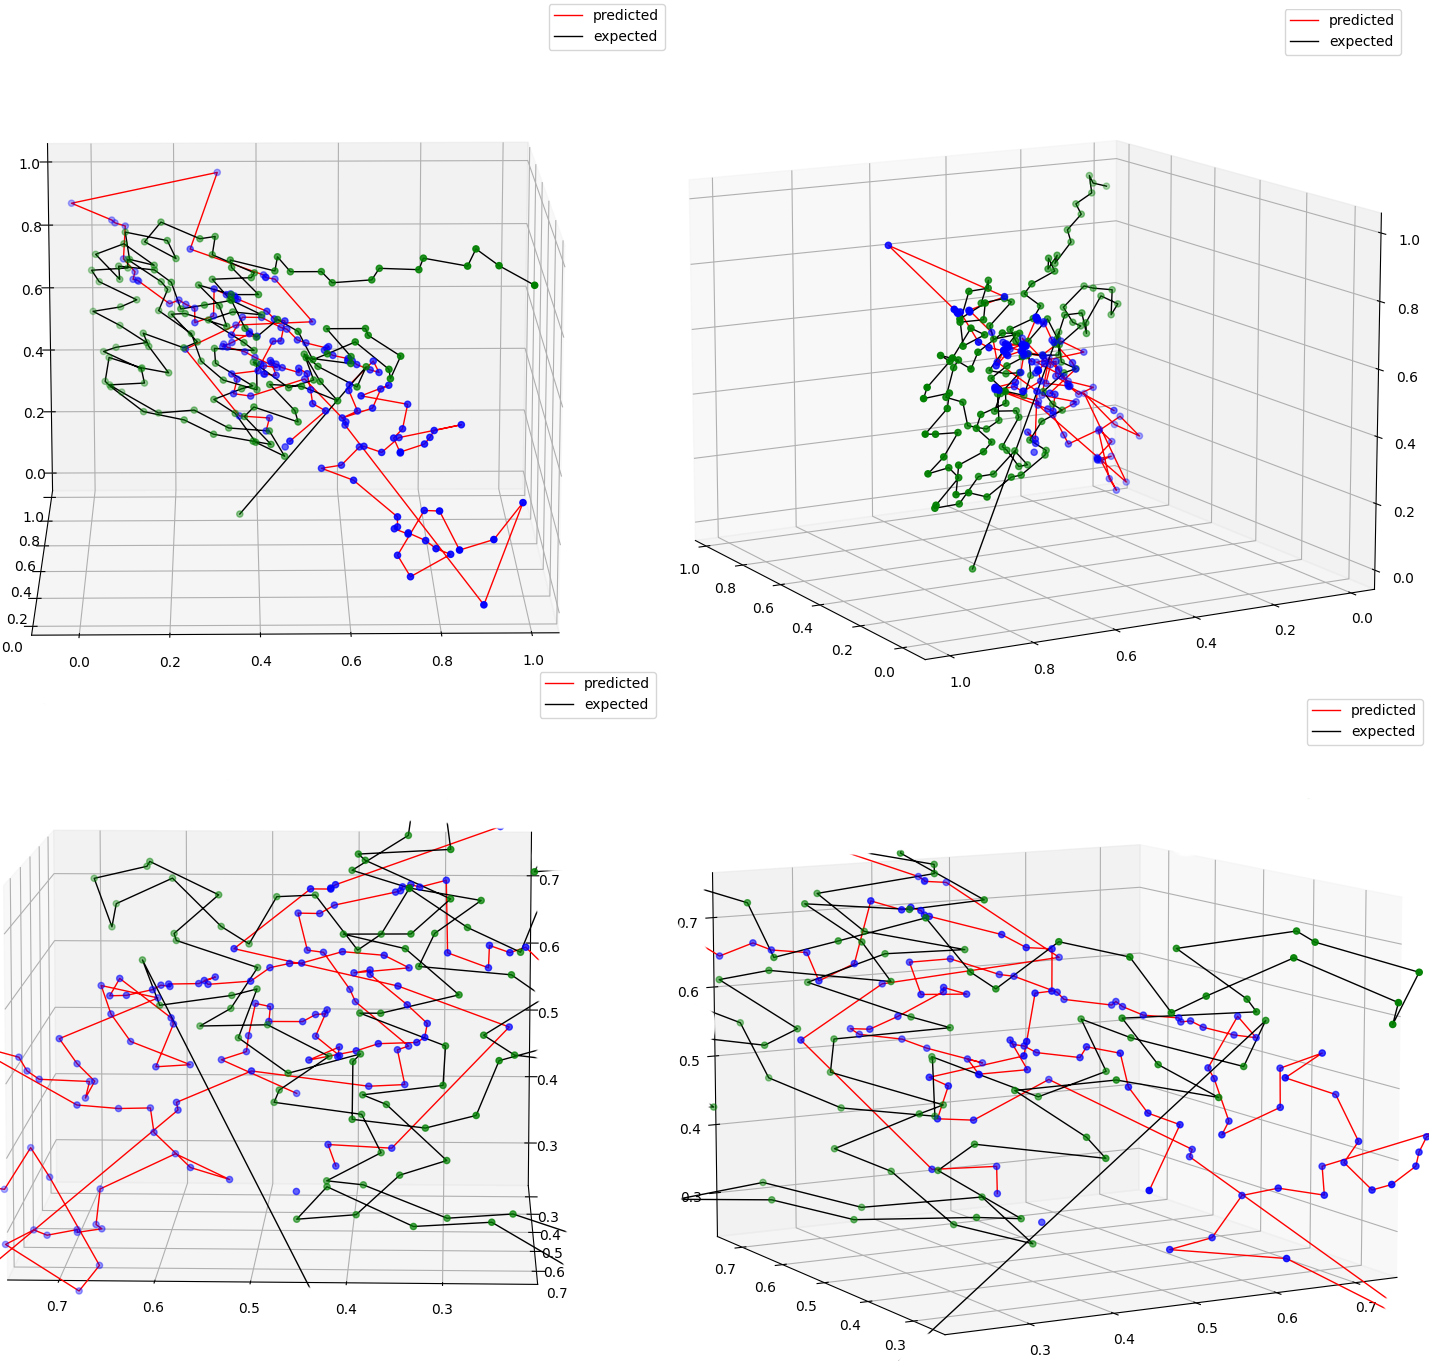
\includegraphics[scale=0.42]{med2.png}\np
\subsection{Poor Prediction}
Loss per sequence: $1.39443$.\\[3mm]
Without reordering:\\[2mm]
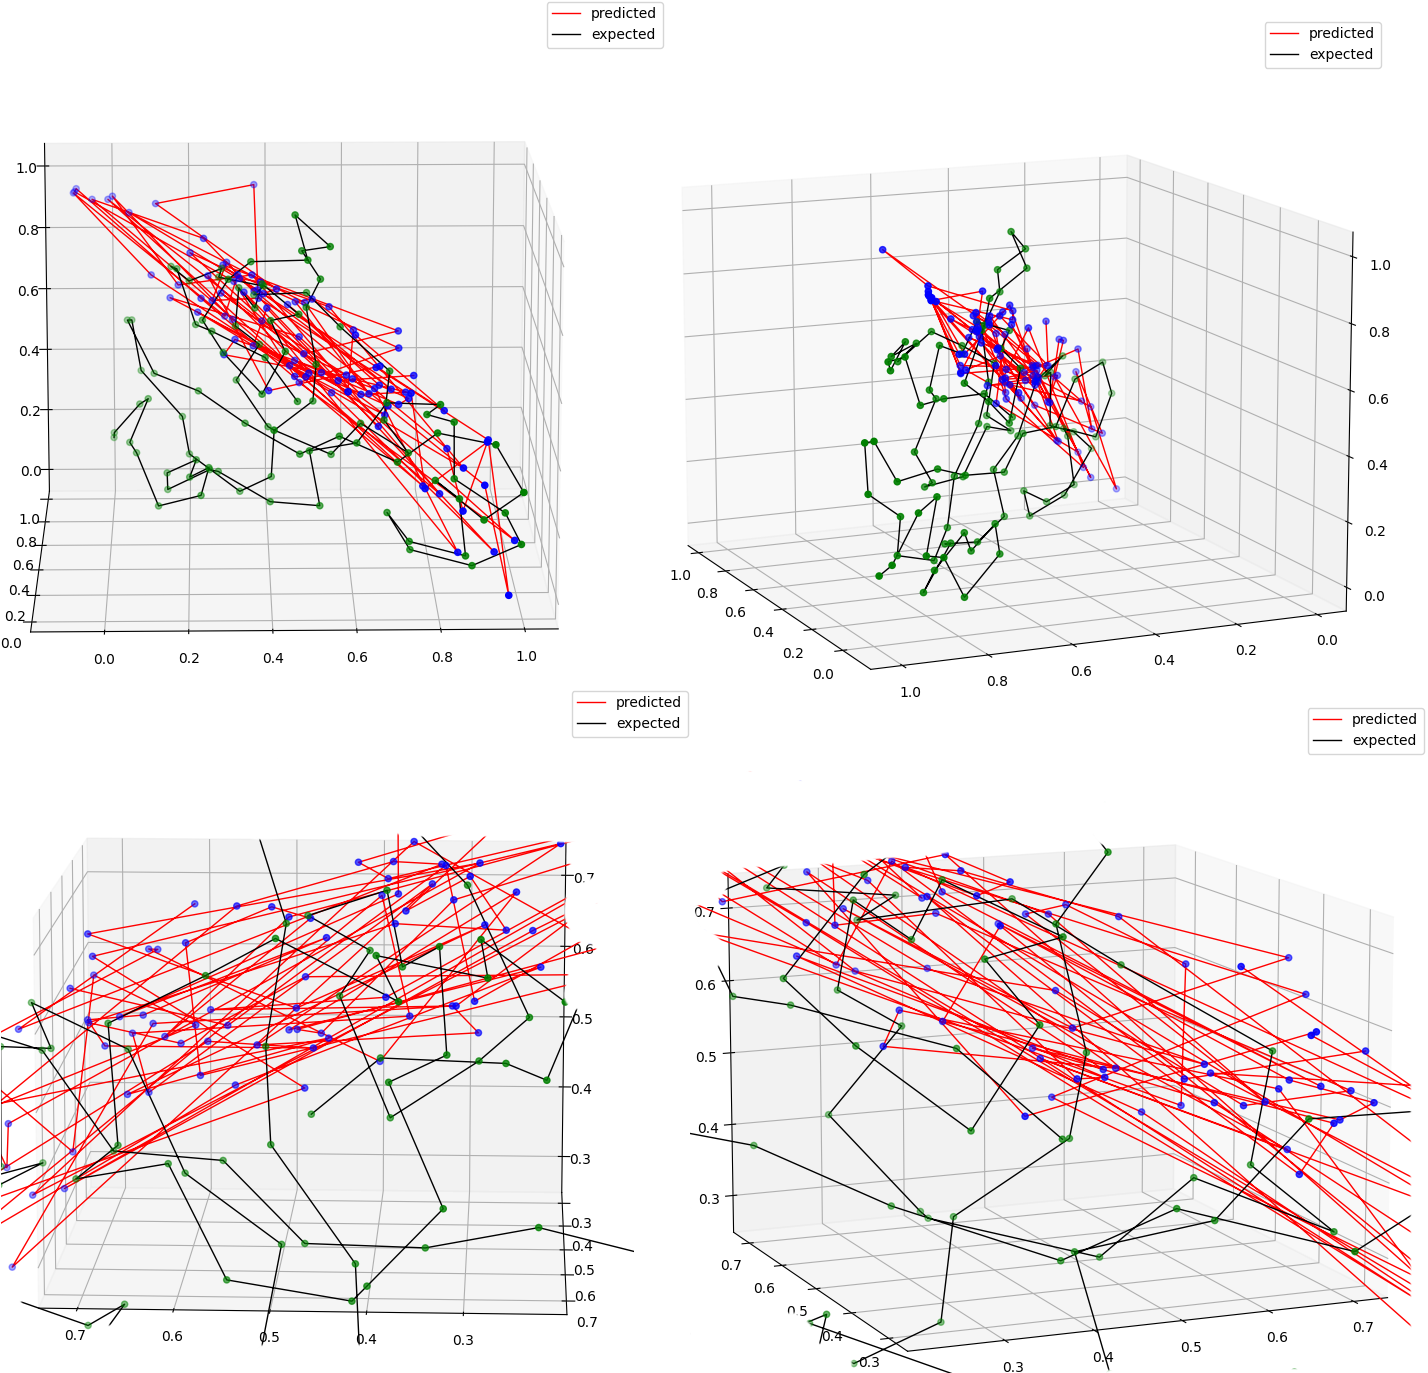
\includegraphics[scale=0.42]{worst1.png}\np
With reordering:\\[2mm]
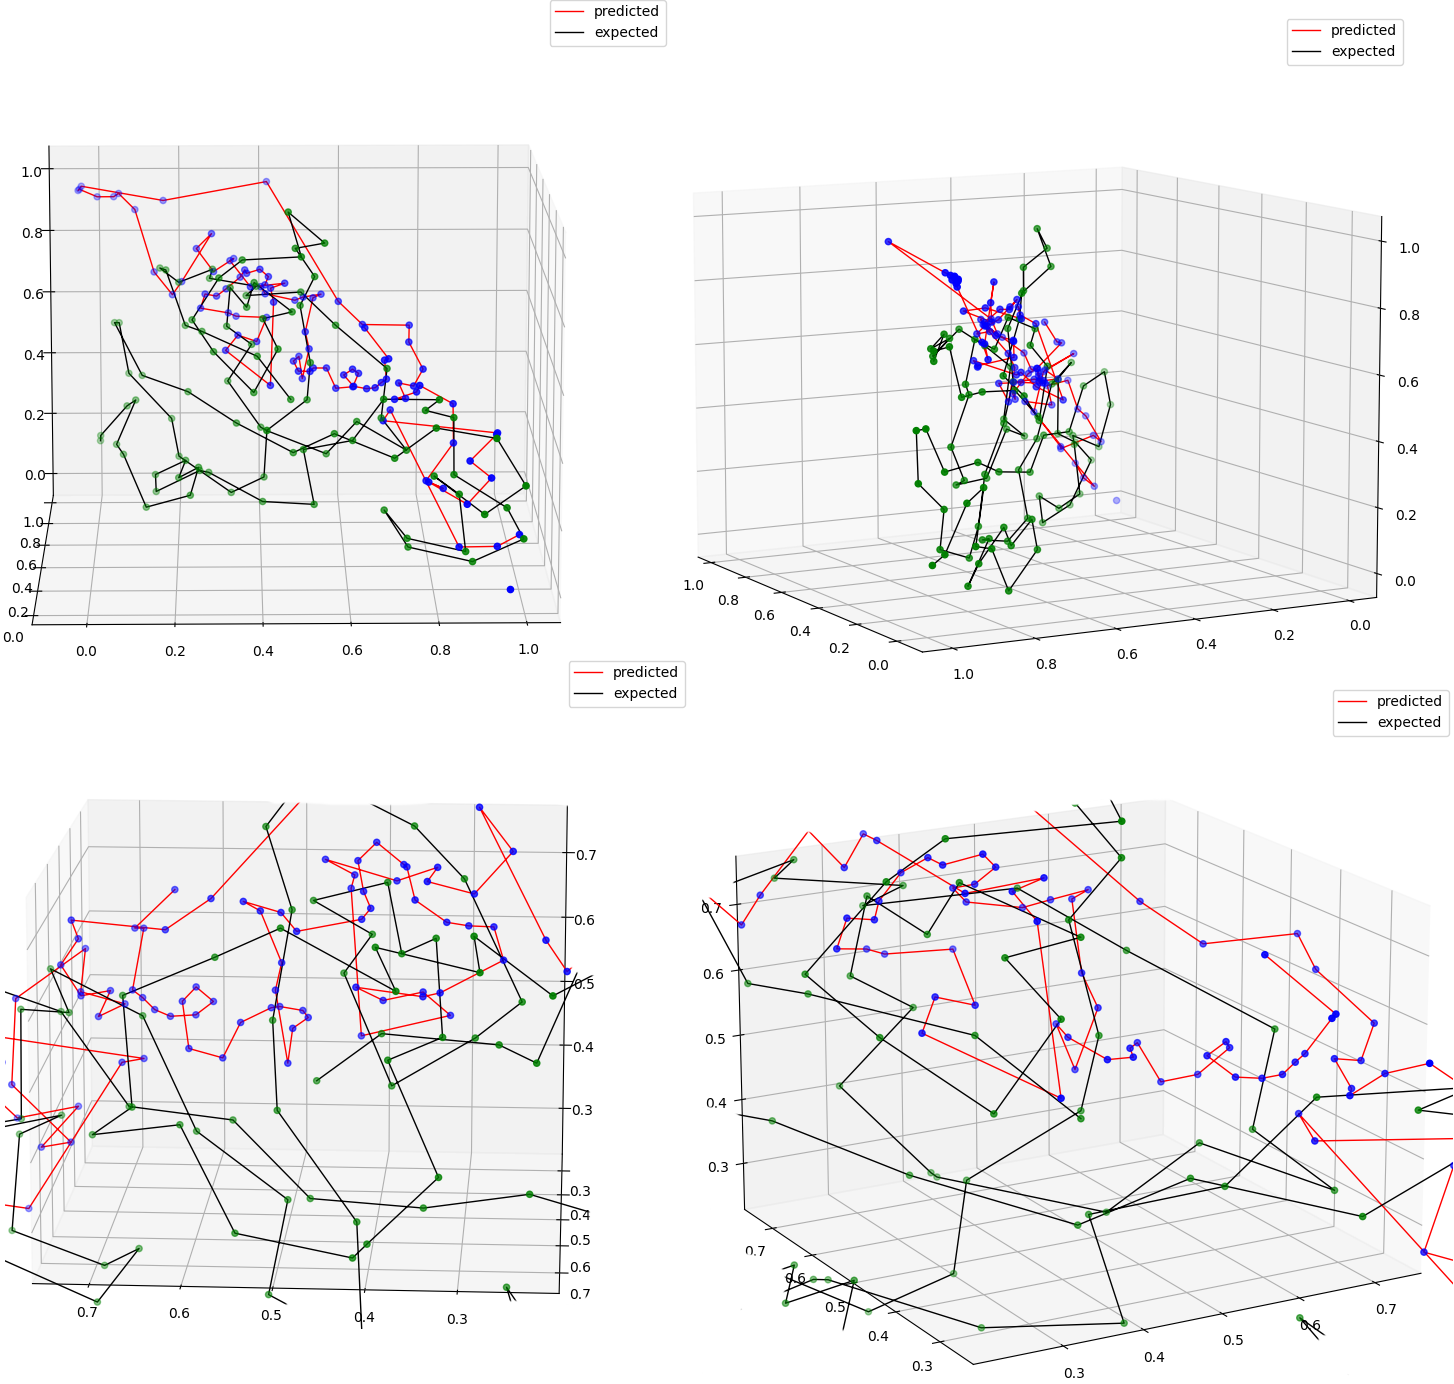
\includegraphics[scale=0.42]{worst2.png}\np

\section{Conclusion}
\subsection{Overall Accuracy}
The 3D-plots above make it evident that the current model is not effective at accurately predicting protein structures.  When the coordinates are normalized, the predicted coordinates of the $C_{\alpha}$ atoms line up reasonably well with the actual coordinates, however the order of the atoms is seemingly random.  When the order is determined post-prediction with the reordering algorithm described above, the prediction appears to match the expected structure better, however it is still far from ideal.

\subsection{Possible Sources of Error}
There are several possible causes for the poor accuracy shown above:
\begin{enumerate}[label=(\alph*)]
	\item The model was not trained for enough time
	\item The model was train with very subpar hyperparameters, leading to very little learning
	\item The reduced dimensionality of the model had a much larger effect on the overall accuracy than was initially expected
	\item There is something fundamentally wrong with the code
\end{enumerate}
Any of these could lead to the inaccurate predictions that the model produces, but most likely it is a combination of all of the above that leads to the poor performance of the model.

\end{document}